\documentclass[12pt, letterpaper]{article}
\usepackage[utf8]{inputenc}
\usepackage[margin=2cm]{geometry}
\usepackage{amsmath}
\usepackage{amssymb}
\usepackage{graphicx}
\usepackage{cancel}
\usepackage{fancyhdr}
\usepackage{float}
\usepackage{mwe,tikz}\usepackage[percent]{overpic}

\graphicspath{ {./bilder/} }

\title{ \begin{huge}
\textbf{Portfolio Assignment 3}
\end{huge} }

\author{Candidate 25}
\date{}

\rfoot{\thepage}
\newcommand{\bs}{\boldsymbol}
\newcommand{\mbf}{\mathbf}

\begin{document}
\maketitle
  \section*{Problem 1}
    \subsection*{(1a)}
      I shall now discuss the main difference between feature extraction and feature selection.\\

      In both feature seletion and extraction the goal is tho reduce the dimensionality of the dataset. Theese are both categories which do this a bit differently. Both algorithms are used to try and avoid the \textit{curse of dimensionality}, a term used to describe the problem of searching for patterns in data which span many features.\\

      In feature extraction we reduce the dimensionality by creating new sets of data, based on the original dataset, this can be done with methods such as principal component analysis or what I am going to do in this problem, multidimensional scaling.\\

      In feature selection we wish to choose features of a dataset which does a good job of describing the dataset as a whole. Sometimes an okay approach to this would be to look at the correlation between features, such that if two features have are highly correlated, only use one of them.\\

      In this problem I implemented a program which used the multidimensional scaling algorithm (MDS), to reduce the number of dimensions in the final output. The way MDS works is by using a result from linear algebra known as eigendecomposition, which uses the eigenvalues and eigenvectors to make what might have began as data structured with 10 features and many datapoints, into data with only 2 or 3 features.\\

      If we define our dataset $X$ we can use eigendecomposition which gives the matrix $E$ which consist of the eigenvectors put together as columnvectors, and the matrix $D$ which is a diagonalmatrix with only eigenvalues on it's main diagonal.
      \begin{align*}
        X^T X = EDE^T &= ED^{1/2}D^{1/2}E^T\\
        \text{IF: } Z &= D^{1/2}E^T\\
        \implies Z^T Z &= X^T X\\
      \end{align*}
      This means we have maximally preserved the inner products and $Z$ is a good representation of $X$. Now we can choose how many
    \subsection*{(1b)}
      In this task we are interested in reducing a 34 x 34 matrix which contains the geodesic distances between 34 swedish cities, into something we can plot on a two dimensional map.\\
      To do this we use MDS and specify that we only want 2 dimensions on the resulting coordinate matrix.\\
    \subsection*{(1c)}
      \begin{figure}[H]
        \caption{Resulting 2 dimensional plot of 34 Swedish cities.}
        \centering
        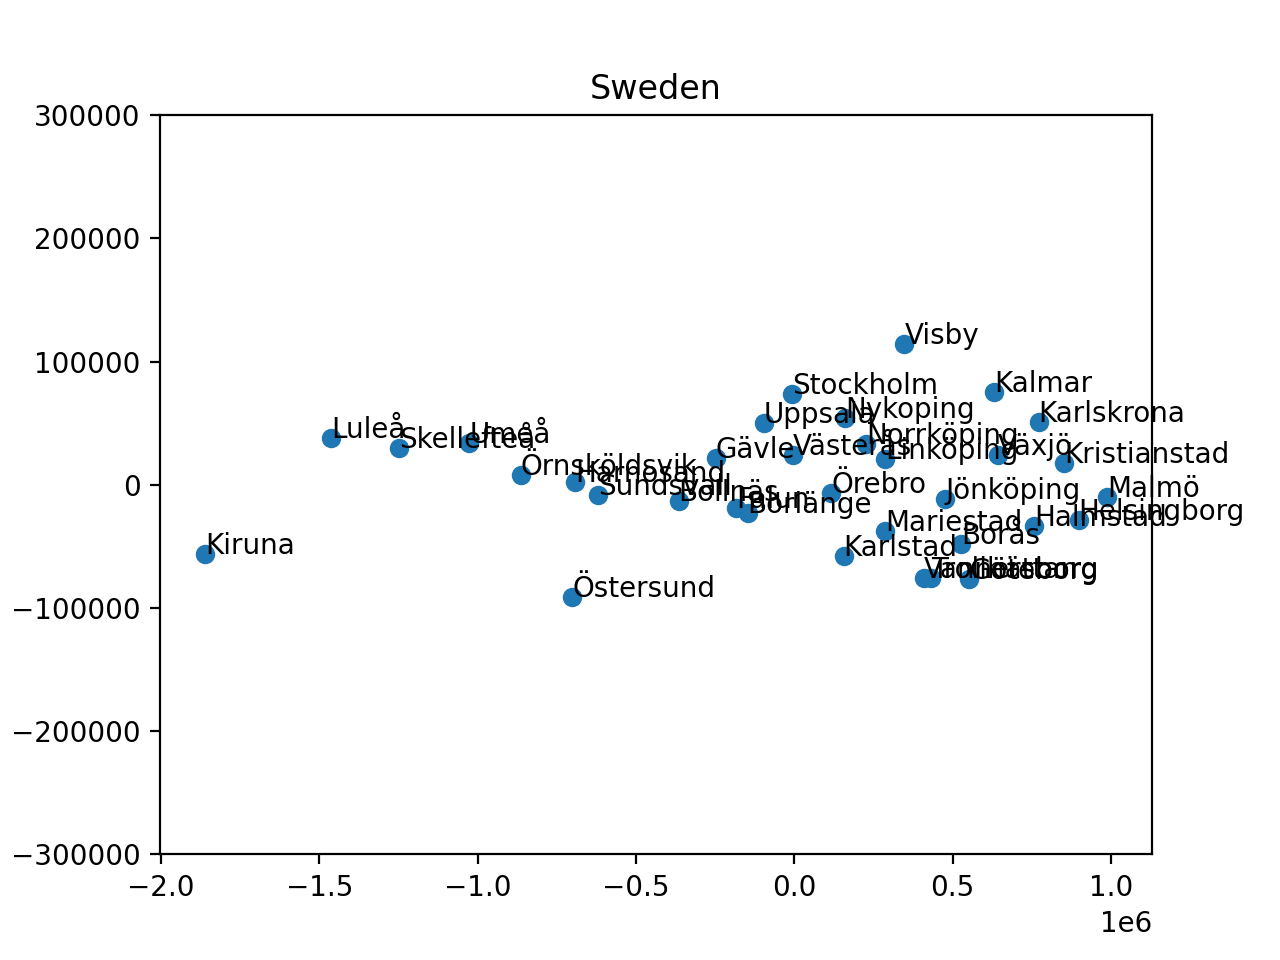
\includegraphics[scale=0.7]{Swedishcities}
        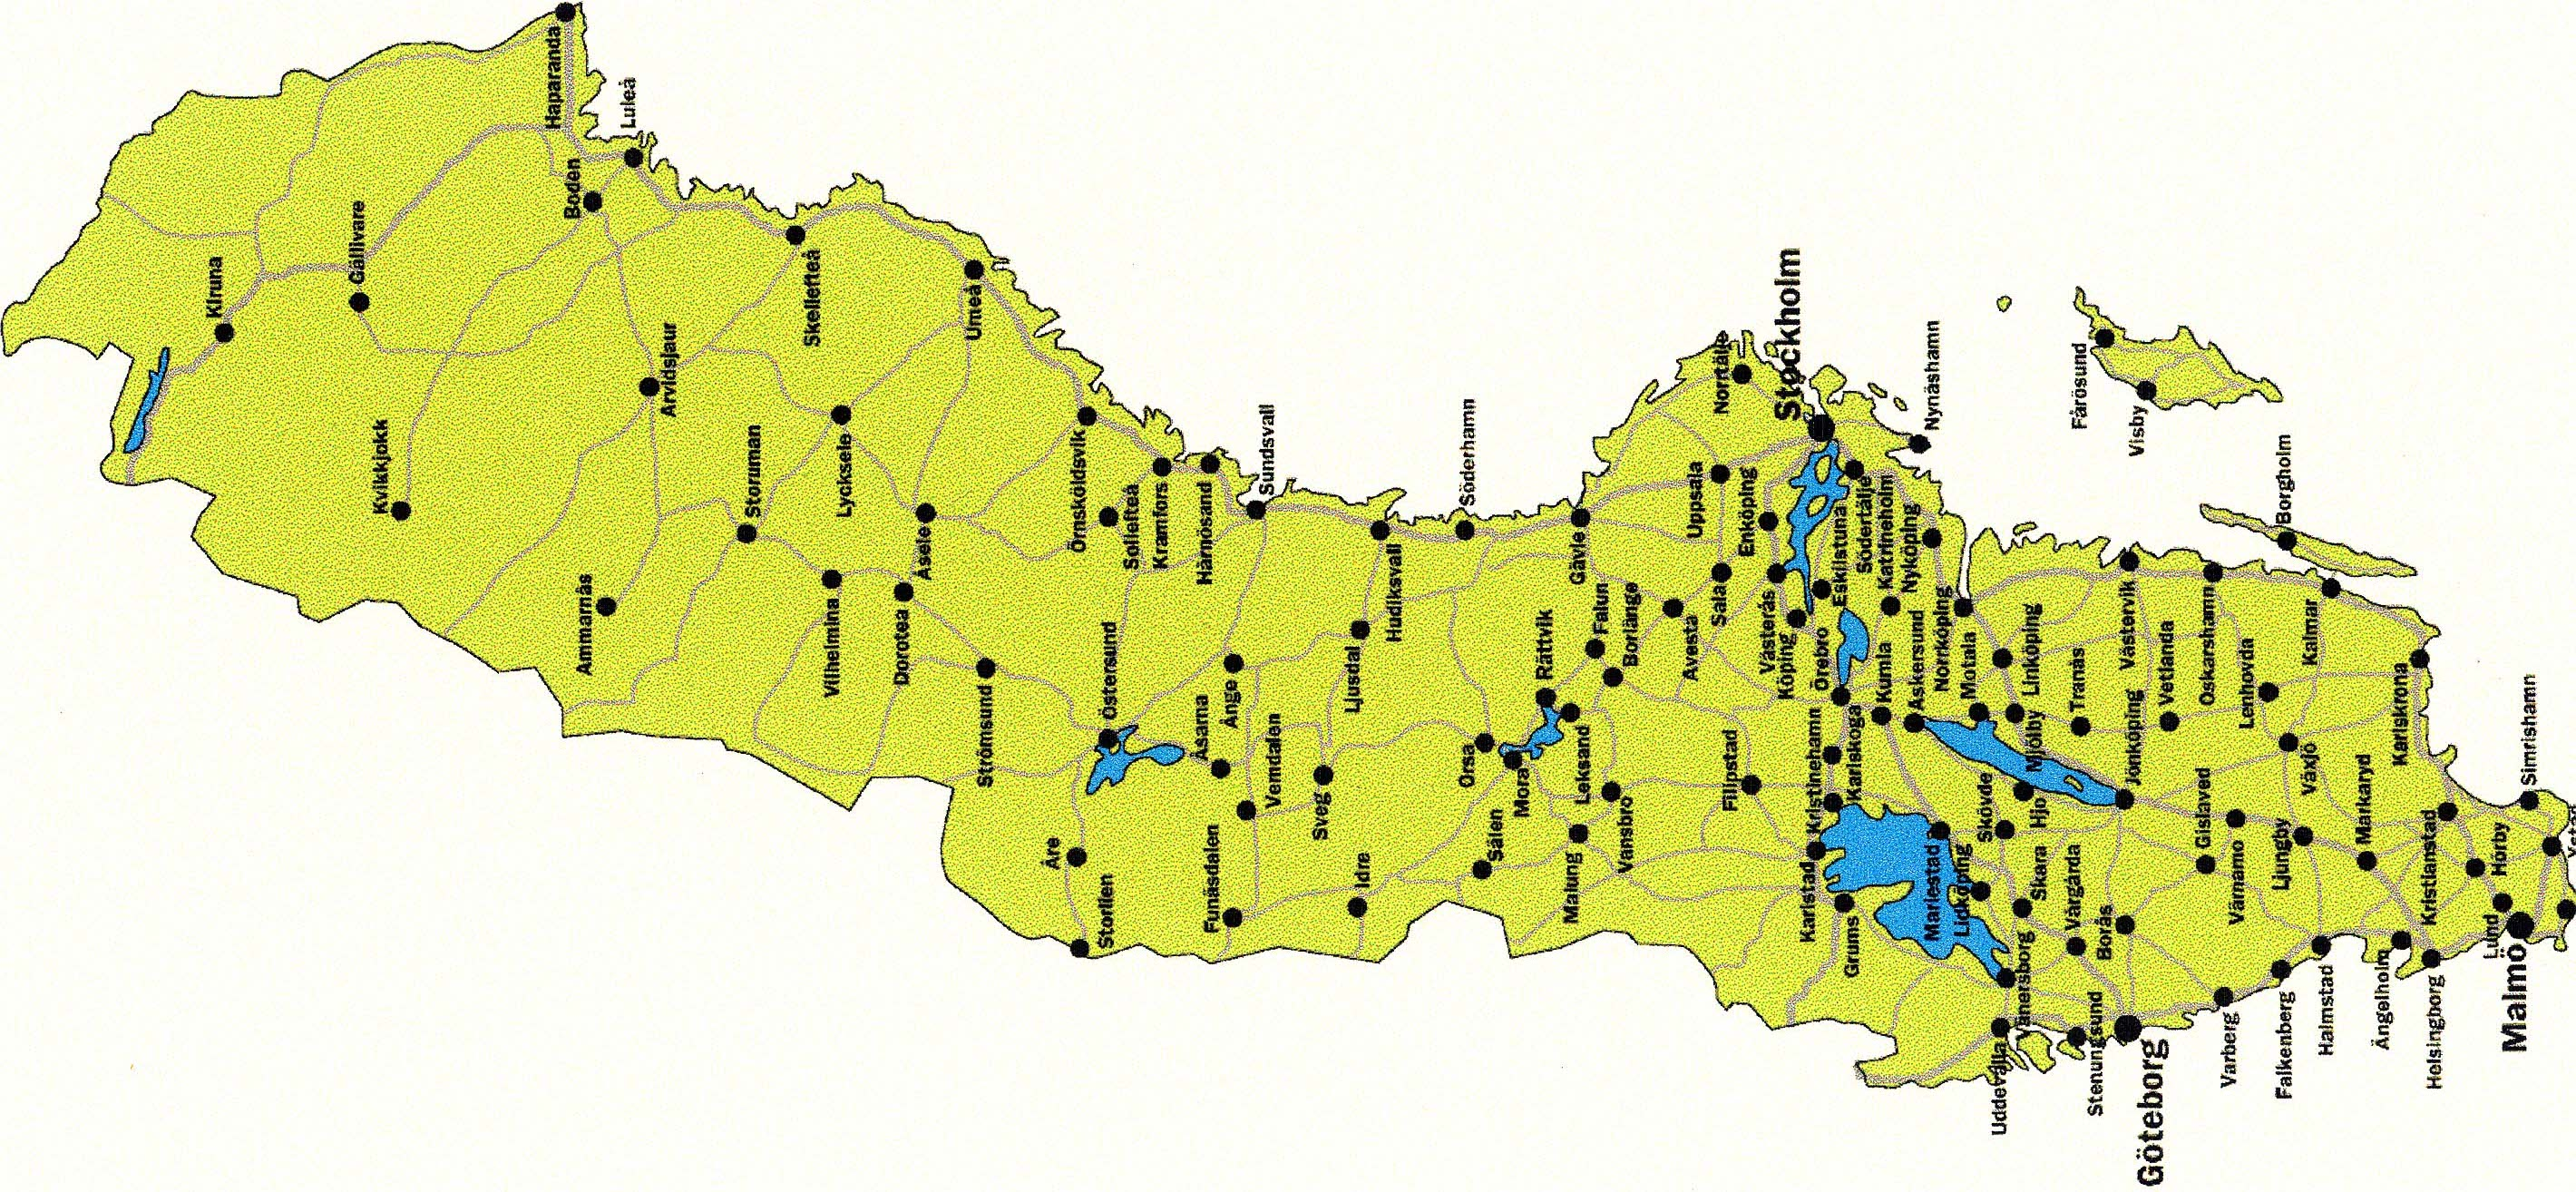
\includegraphics[scale=0.1]{Swedishmap}
      \end{figure}\\
  \section*{Problem 2}
    \subsection*{(2a)}
      \begin{figure}[H]
        \caption{}
        \centering
        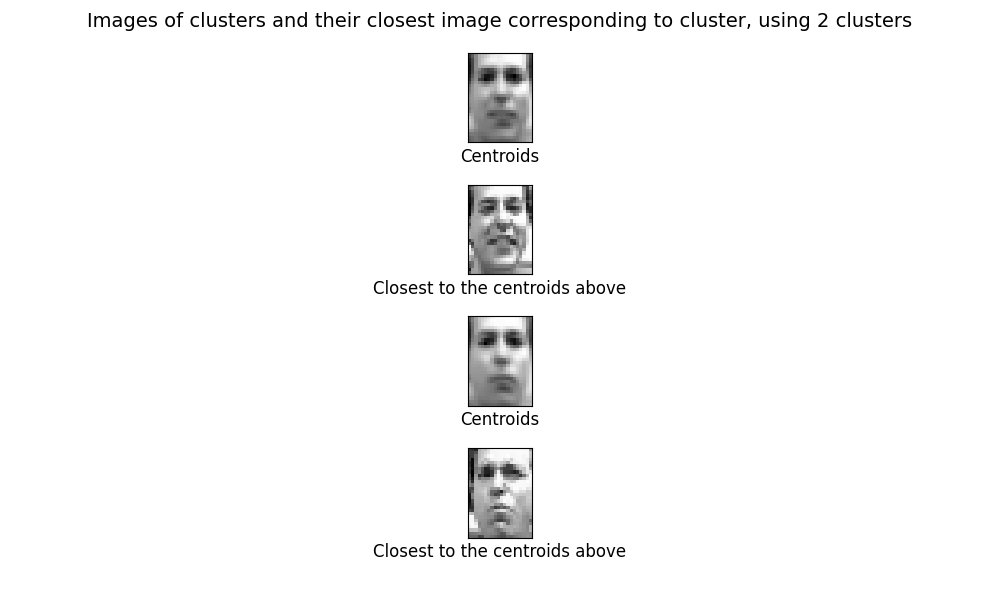
\includegraphics[scale=0.7]{cluster2}
        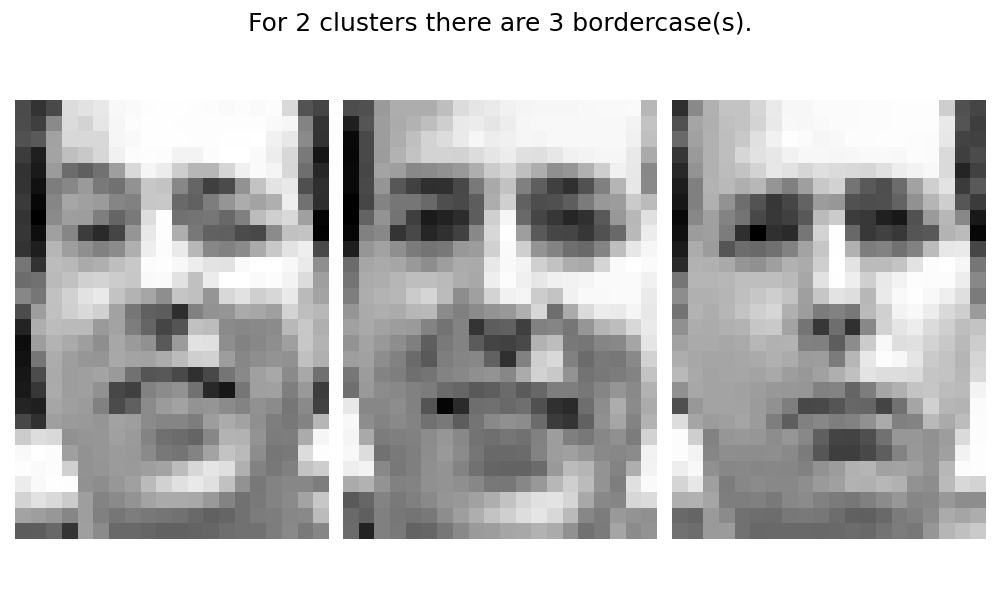
\includegraphics[scale=0.4]{border2}
      \end{figure}\\
      \begin{figure}[H]
        \caption{}
        \centering
        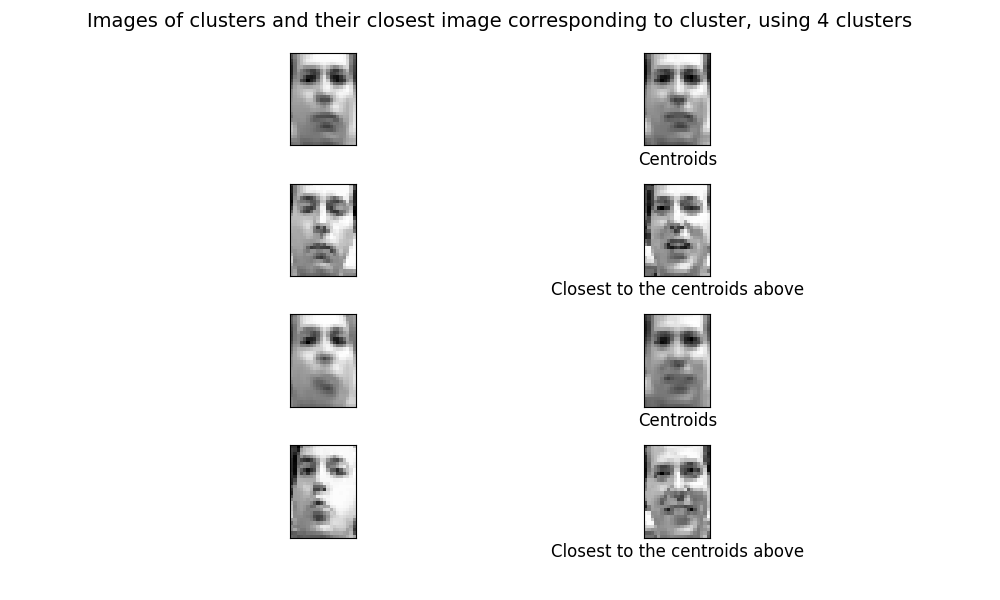
\includegraphics[scale=0.7]{cluster4}
        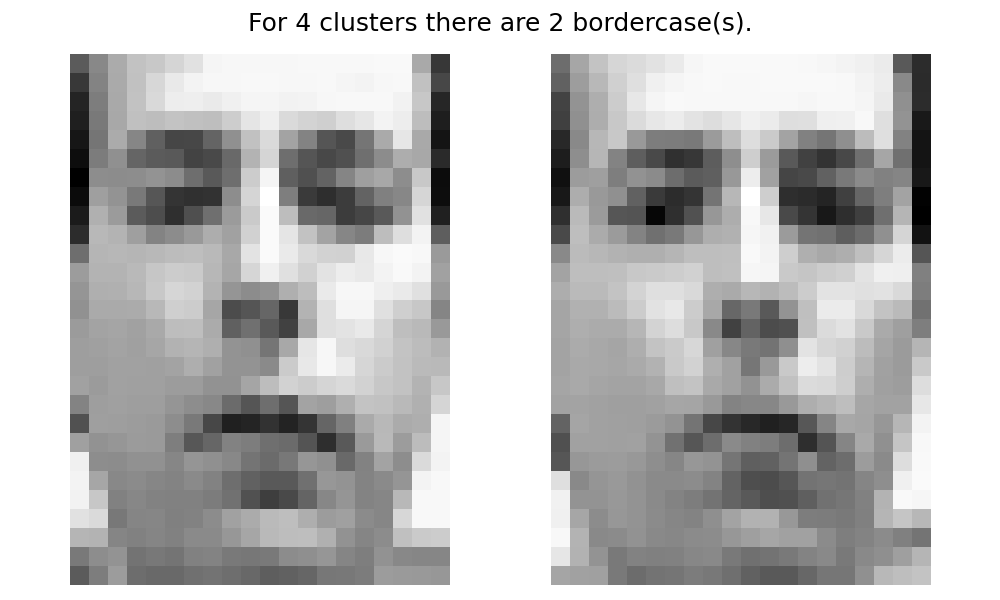
\includegraphics[scale=0.4]{border4}
      \end{figure}\\
      \begin{figure}[H]
        \caption{}
        \centering
        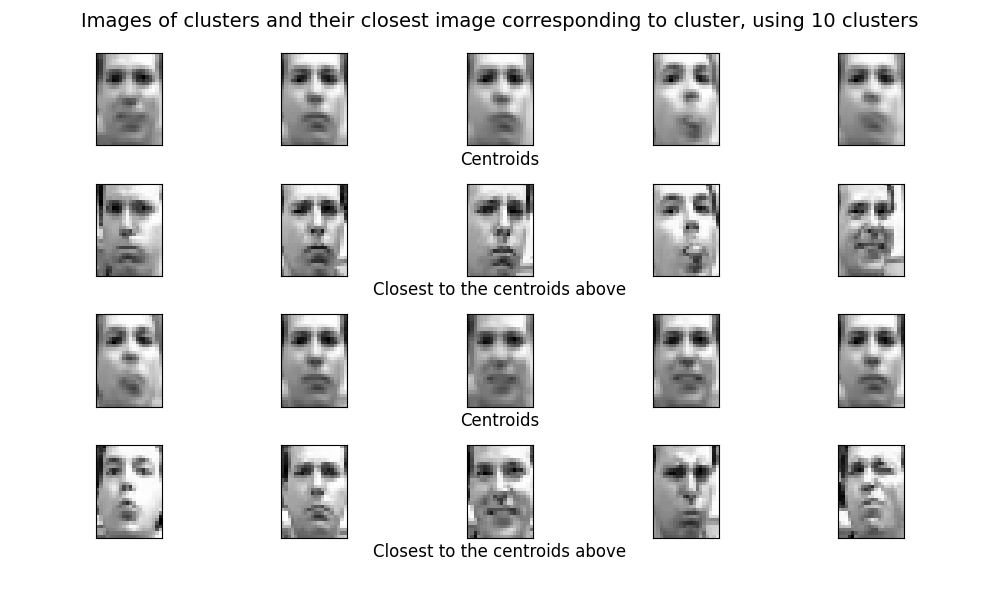
\includegraphics[scale=0.7]{cluster10}
        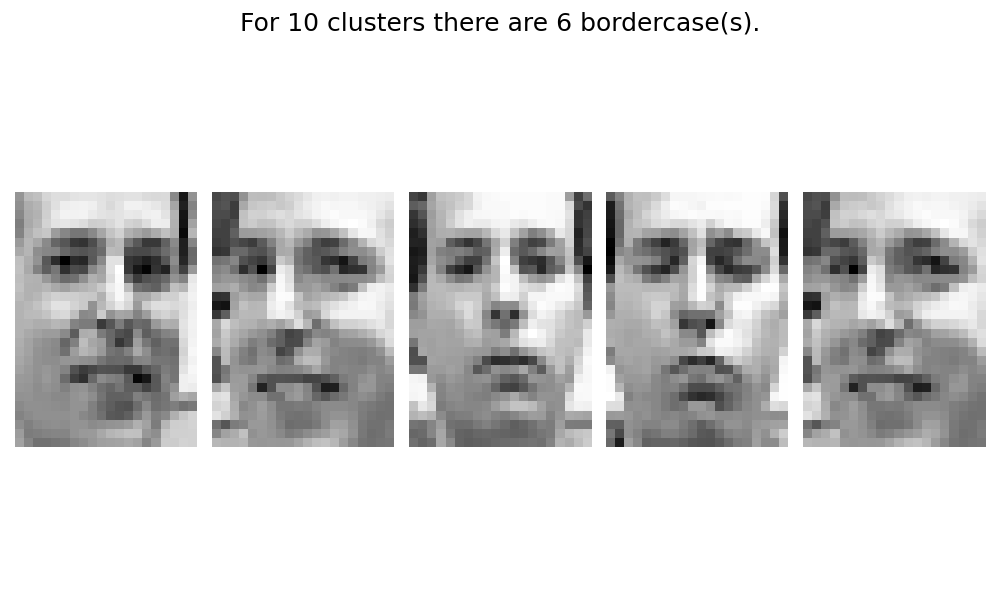
\includegraphics[scale=0.4]{border10}
      \end{figure}\\
    \subsection*{(2b)}
    \subsection*{(2c)}
\end{document}
